%----------------------------------------------------------------------------------------
%	PACKAGES AND DOCUMENT CONFIGURATIONS
%----------------------------------------------------------------------------------------
\documentclass[11pt]{article}
\usepackage{amsmath} % Required for some math elements
\usepackage{hyperref} 
\usepackage{xcolor}
\usepackage{lipsum} 
\usepackage{cite}
\usepackage{graphicx} % Required for the inclusion of images
\usepackage{algorithmic}
\usepackage{array}
\usepackage{bookmark}
\usepackage{listings}
\usepackage{amssymb}
\usepackage{enumitem}
\usepackage[margin=8mm]{geometry}
\usepackage[caption=false, font=footnotesize]{subfig}
\usepackage{fancyhdr}
\pagestyle{fancy}
\lhead{ENGR222 Assignment 1 Submission}
\rhead{Daniel Eisen : 300447549}
\cfoot{\thepage}
\renewcommand{\headrulewidth}{0.4pt}
\renewcommand{\footrulewidth}{0.4pt}
\usepackage[active,tightpage]{preview}

\renewcommand{\PreviewBorder}{1in}

\newlist{steps}{enumerate}{1}
\setlist[steps, 1]{label = Step \arabic*:}

\hypersetup{ %color attributes of citation, link, etc.
    colorlinks=true,
    linkcolor=blue,
    filecolor=gray,      
    urlcolor=blue,
    citecolor=blue,
}

\newcommand{\matlab}{\textsc{Matlab }} %very important and totally necessary addition
 
\newcommand\Item[1][]{%
  \ifx\relax#1\relax  \item \else \item[#1] \fi
  \abovedisplayskip=0pt\abovedisplayshortskip=0pt~\vspace*{-\baselineskip}}
%----------------------------------------------------------------------------------------
%	DOCUMENT INFORMATION
%----------------------------------------------------------------------------------------

\title{ENGR 222 \\ Assignment 2 Submission}
\author{Daniel Eisen : 300447549}
\date{\today}

\begin{document}
\begin{preview}

    \maketitle
    %----------------------------------------------------------------------------------------
    %	DOCUMENT CONTENT
    %----------------------------------------------------------------------------------------

    \begin{enumerate}
        \item \textbf{Multivariate Function}
              $$f(x,y) = -2x^{3} + 3x^{2}y + 2y^{3} - 9y + 5$$
              \begin{enumerate}
                  \Item
                  \begin{align*}
                      f_{x} & = -6x^{2} + 6xy       \\
                      f_{y} & = 3x^{2} + 6y^{2} - 9 \\
                  \end{align*}
                  \Item
                  \begin{align*}
                      f_{xy} & = 6x        \\
                      f_{xx} & = -12x + 6y \\
                      f_{yy} & = 12y       \\
                  \end{align*}
                  \Item
                  \begin{align*}
                      f_x                              & = -6x^{2} + 6xy = 0                                  \\
                      f_y                              & = 3x^{2} + 6y^{2} - 9 = 0                            \\
                      \mathrm{by \; inspection \;}  (x & =y=1,-1)                                             \\
                      for \; x=0,                                                                             \\
                      f_x                              & = 0                                                  \\
                      f_y                              & = 6y^2 - 9 = 0                                       \\
                      \therefore \; y = \sqrt{9/6}     & = \sqrt{\frac{3}{2}}                                 \\
                      for \; y=0:                                                                             \\
                      f_x                              & = -6x^2 = 0                                          \\
                      f_y                              & = 3x^2 - 9 = 0                                       \\
                      \mathrm{no \; x}                                                                        \\
                      \mathrm{critical \; points}      & \Rightarrow [(1,1), (-1,-1), (0,\sqrt{\frac{3}{2}})] \\
                  \end{align*}
                  \Item Second Partials test:
                  \begin{align*}
                      D                                        & = f_{xx}(0,\sqrt{\frac{3}{2}}) \cdot f_{yy}(0,\sqrt{\frac{3}{2}}) - f^2_{xy}(0,\sqrt{\frac{3}{2}}) \\
                      f_{xx} = -12x + 6y, f_{yy} = 12y, f_{xy} & = 6x                                                                                               \\
                      D                                        & = (-12(0) + 6\left(\sqrt{\frac{3}{2}}\right))(12\left(\sqrt{\frac{3}{2}}\right)) - (6(0))^2        \\
                                                               & = (0 + 3\sqrt{6})(6\sqrt{6})-0                                                                     \\
                                                               & =    108
                  \end{align*}
                  $D>0$ and $f_{xx} > 0$ therefore, this critical point is a local minimum.
              \end{enumerate}

              \newpage
        \item \textbf{Quick questions}
              \begin{enumerate}
                  \Item
                  $f(x,y,z) = e^{x}cos(y)(1-z)^{2}, \; \textbf{u} = (0.36, 0.48, 0.8)$ \\
                  \begin{align*}
                      D_{\textbf{\textbf{u}}} & = f_{x}u_{1} + f_{y}u_{2} + f_{z}u_{3} \\ \\
                      f_{x}                   & = e^{x}cos(y)(1-z)^{2}                 \\
                      f_{x}(0,0,0)            & = 1 \times 1 \times 1 = 1              \\
                      f_{y}                   & = -e^{x}sin(y)(1-z)^2                  \\
                      f_{y}(0,0,0)            & = -1 \times 0 \times 1 = 0             \\
                      f_{z}                   & = 2e^{x}cos(y)(z - 1)                  \\
                      f_{z}(0,0,0)            & = 2 \times 1 \times -1 = -2            \\ \\
                      D_{\textbf{\textbf{u}}} & = 1(0.36) + 0(0.48) + -2(0.8)=-1.24    \\
                  \end{align*}
                  \Item
                  $f(x,y,z) = (1+x)(1-y^2)(1-z)^2, \; \textbf{p} = (1,2,3) $\\
                  \begin{align*}
                      L(x,y,z)          & = f(x_0, y_0, z_0) + f_x(x_0, y_0, z_0)(x-x_0) \\
                                        & + f_y(x_0, y_0, z_0)(y-y_0)                    \\
                                        & + f_z(x_0, y_0, z_0)(z-z_0)                    \\\\
                      f(\textbf{p})     & = (1+1)(1-2^2)(1-3)^2=-24                      \\ \\
                      f_{x}             & = (1-y^2)(1-z)^2                               \\
                      f_{x}(\textbf{p}) & = (1-2^2)(1-3)^2=-12                           \\
                      f_{y}             & = (1+x)(-2y)(1-z)^2                            \\
                      f_{y}(\textbf{p}) & = (1+1)(-2(2))(1-3)^2=-32                      \\
                      f_{z}             & = 2(1+x)(1-y^2)(z-1)                           \\
                      f_{z}(\textbf{p}) & = 2(1+1)(1-2^2)(3-1)=-24                       \\\\
                      L(\textbf{p})     & = -24 + (-12)(x-1) + (-32)(y-2) + (-24)(z-3)   \\
                                        & = 124 - 12x - 32y - 24z
                  \end{align*}
                  \Item $f(x,y) = e^{-x^2-y^2} = e^{-x^2}e^{-y^2}, \; \textbf{p} = (1,1) $\\
                  \begin{align*}
                      L(x,y)     & =  f(\textbf{p}) + f_x(\textbf{p})(x-x_0)+ f_y(\textbf{p})(y-y_0)                                                                    \\
                      p_{2}(x,y) & = L(x,y) + \frac{1}{2}\left[(x-x_0)^{2}f_{xx}(\textbf{p}) + 2(x-x_0)(y-y_0)f_{xy}(\textbf{p}) + (y-y_0)^{2}f_{yy}(\textbf{p})\right] \\
                  \end{align*}
                  \begin{align*}
                      f_{x}              & = -2xe^{-x^2}e^{-y^2}                                                                                 \\
                                         & = -2xe^{-x^2-y^2}                                                                                     \\
                      f_{y}              & = -2ye^{-x^2}e^{-y^2}                                                                                 \\
                                         & = -2ye^{-x^2-y^2}                                                                                     \\\\
                      f_{xx}             & = e^{-y^2}(-2(e^{-x^2}) + -2x(-2xe^{-x^2}))                                                           \\
                                         & = (4x^2 - 2)e^{-x^2-y^2}                                                                              \\
                      f_{yy}             & = (4y^2 - 2)e^{-x^2-y^2}                                                                              \\
                      f_{xy}             & = -2xe^{-x^2}(-2ye^{-y^2})                                                                            \\
                                         & = 4xye^{-x^2-y^2}                                                                                     \\\\
                      f(\textbf{p})      & = e^{-1^2-1^2} = e^{-2}                                                                               \\
                      f_{x}(\textbf{p})  & = -2e^{-1^2-1^2} = -2e^{-2}                                                                           \\
                      f_{y}(\textbf{p})  & = -2e^{-1^2-1^2} = -2e^{-2}                                                                           \\
                      f_{xx}(\textbf{p}) & = (4(1^2) - 2)e^{-1^2-1^2} = 2e^{-2}                                                                  \\
                      f_{yy}(\textbf{p}) & = (4(1^2) - 2)e^{-1^2-1^2} = 2e^{-2}                                                                  \\
                      f_{xy}(\textbf{p}) & = 4e^{-1^2-1^2} = 4e^{-2}                                                                             \\\\
                      L(\textbf{p})      & = e^{-2} + -2e^{-2}(x-1) + -2e^{-2}(y-1) = (5-2x-2y)e^{-2}                                            \\
                      p_{2}(\textbf{p})  & = (5-2x-2y)e^{-2} + \frac{1}{2}\left[ (x-1)^{2}2e^{-2} + (x-1)(y-1)8e^{-2} + (y-1)^{2}2e^{-2} \right] \\
                                         & = (5-2x-2y)e^{-2} + \left((x-1)^{2} + 4(x-1)(y-1)e^{-2} + (y-1)^{2}\right)e^{-2}                      \\
                                         & = \left(x^2+y^2+4xy-8x-8y+11\right)e^{-2}                                                             \\
                  \end{align*}
                  \Item $f(x,y) = x^{3} + y^{3} - 4x - 2y + 1 ,\; (x(t), y(t)) = (t^{3}-2t, t^{2})$\\\\
                  \begin{align*}
                      \nabla f(x,y)  & = f_{x}(x,y)\textbf{i} + f_{y}(x,y)\textbf{j}         \\\\
                      f_{x}          & = 3x^{2} - 4                                          \\
                      f_{y}          & = 3y^{2} - 2                                          \\
                      \nabla f(x,y)  & = (3x^{2} - 4)\textbf{i} + (3y^{2} - 2)\textbf{j}     \\\\
                      (x(1), y(1))   & = (-1, 1)                                             \\
                      \nabla f(-1,1) & = (3(-1^2) - 4)=-1\textbf{i} + (3(1^2) - 2)\textbf{j} \\
                                     & = -\textbf{i} + \textbf{j}                            \\
                  \end{align*}
                  \Item $z = x^2 + xy - y^4, \; \textbf{p} = (2,1)$ \\
                  \begin{align*}
                      \mathrm{find \; z \; at (2,1): \;} &                                                                                       \\
                      z                                  & = 2^2 + 2 - 1 = 5                                                                     \\
                      F(x,y,z)                           & = z - x^2 - xy + y^4 = 0, \; \textbf{p} = (2,1,5)                                     \\
                      \nabla F(x,y,z)                    & = (-2x - y)\textbf{i} + (4y^3 - x)\textbf{j} + \textbf{k}                             \\
                      \nabla F(\textbf{p})               & = (-2(2) - 1)\textbf{i} + (4(1^3) - 2)\textsubscript{j} + \textbf{k}                  \\
                                                         & = -5\textbf{i} + 2\textsubscript{j} + \textbf{k}                                      \\
                      \mathrm{tangent \; plane}          & = \nabla F(\textbf{p}) \cdot (\textbf{v} - \textbf{p}) = 0 \; : \; \textbf{v}=(x,y,z) \\
                                                         & = -5(x-2) + 2(y-1) + (z-5) = 0                                                        \\
                                                         & = -5x + 2y + z= -3 \; \mathrm{or} \; z = 5x -2y -3                                    \\
                  \end{align*}
              \end{enumerate}
        \item \textbf{Double integrals}
              \begin{enumerate}
                  \Item $e^{-x}cos(y)$ \\
                  \begin{align*}
                       & \int_{\pi/2}^{-\pi/2} \int_{0}^{2} e^{-x}cos(y) \,dx  \,dy           \\
                       & =  \int_{\pi/2}^{-\pi/2} cos(y) \int_{0}^{2} e^{-x} \,dx  \,dy       \\
                       & =  \int_{\pi/2}^{-\pi/2} cos(y) \Big| -e^{-x} \Big|_{x=0}^{x=2} \,dy \\
                       & =  \int_{\pi/2}^{-\pi/2} cos(y) \left(-e^{-2} - -e^{-0}\right) \,dy  \\
                       & =  \int_{\pi/2}^{-\pi/2} (1-e^{-2})cos(y) \,dy                       \\
                       & =  (1-e^{-2}) \Big| sin(y) \Big|_{y=\pi/2}^{y=-\pi/2}                \\
                       & =  (1-e^{-2}) (sin(\pi/2) - sin(-\pi/2))                             \\
                       & =  2(1-e^{-2}) = 2-2e^{-2}                                           \\
                  \end{align*}
                  \Item $f(x, y) = sin(x+y), \; R : x,y \ge 0, x+y \le \pi$\\\\
                  \begin{align*}
                       & \int_{0}^{\pi} \int_{0}^{\pi-y} sin(x+y) \,dx  \,dy                                                  \\
                       & = \int_{0}^{\pi} \Big| -cos(x+y) \Big|_{x=0}^{x=\pi-y}  \,dy                                         \\
                       & = \int_{0}^{\pi} (-cos(\pi-y+y) + cos(0+y))  \,dy                                                    \\
                       & = \int_{0}^{\pi} (-cos(\pi) + cos(y))  \,dy                                                          \\
                       & = \int_{0}^{\pi} 1 + cos(y) \,dy = \Big| y + sin(y) \Big|_{0}^{\pi} = (\pi + sin(\pi) -  0 - sin(0)) \\
                       & = \pi
                  \end{align*}
                  \Item
                  \begin{align*}
                      |R| & = \int_{0}^{5} \int_{e^{y/3}}^{10+sin(y)} 1 \,dx  \,dy  \\
                          & = \int_{0}^{5} \int_{e^y/3}^{10+sin(y)} 1 \,dx  \,dy    \\
                          & = \int_{0}^{5} \Big| x \Big|_{e^{y/3}}^{10+sin(y)} \,dy \\
                          & = \int_{0}^{5} \Big| x \Big|_{e^{y/3}}^{10+sin(y)} \,dy \\
                          & = \int_{0}^{5} 10+sin(y) - e^{y/3} \,dy                 \\
                          & = \Big| 10y-cos(y) - 3e^{y/3} \Big|_{0}^{5} \,dy        \\
                          & = (50-cos(5) - 3e^{5/3}) - (0-cos(0) - 3e^{0})          \\
                          & \approx 37.83286..
                  \end{align*}
                  \Item $f(x,y) = 3y - 2x, \; R = \{(x,y):0 \le y \le 4-x^2, x \in [-2,2]\}$ \\\\
                  \begin{align*}
                      \mu & = \frac{1}{|R|} \int \int_R f(x,y) \,dA                                                    \\\\
                      |R| & = \int_{-2}^{2} \int_{0}^{4-x^{2}} 1 \,dy  \,dx                                            \\
                          & = \int_{-2}^{2} \Big| y \Big|_{y=0}^{y=4-x^{2}} \,dx                                       \\
                          & = \int_{-2}^{2} 4-x^{2} \,dx                                                               \\
                          & = \Big| 4x-\frac{x^{3}}{3} \Big|_{x=-2}^{x=2}                                              \\
                          & = (4(2)-\frac{2^{3}}{3}) - (4(-2)-\frac{(-2)^{3}}{3}) = \frac{32}{3}                       \\\\
                          & \int_{-2}^{2} \int_{0}^{4-x^{2}} 3y - 2x \,dy  \,dx                                        \\
                          & \int_{-2}^{2} \Big| \frac{3}{2}y^2 - 2xy \Big|_{y=0}^{y=4-x^{2}}  \,dx                     \\
                          & \int_{-2}^{2} \frac{3}{2}(4-x^{2})^2 - 2x(4-x^{2})  \,dx                                   \\
                          & \int_{-2}^{2} \frac{3x^4}{2}+2x^3-12x^2-8x+24 \,dx                                         \\
                          & \Big| \frac{3x^5}{10}+\frac{2x^4}{4}-\frac{12x^3}{3}-\frac{8x^2}{2}+24x \Big|_{x=-2}^{x=2} \\
                          & = 256/5 = 51.2                                                                             \\\\
                      \mu & = \frac{256/5}{32/3} = 4.8                                                                 \\
                  \end{align*}
                  \Item $z=\sqrt{9-x^{2}}, \; R = \{(x,y) : 0 \le y \le x, x \in [0,3]\}$ \\\\
                  \begin{align*}
                      \mathrm{surface \; area} & = \int \int_R \sqrt{(f_{x})^2 + (f_{y})^2 +1} \, dA                                           \\
                                               & = \int_{0}^{3} \int_{0}^{x} \sqrt{\left(-\frac{x}{\sqrt{9-x^2}}\right)^2 + 0^2 + 1} \,dy \,dx \\
                                               & = \int_{0}^{3} \int_{0}^{x} \frac{3}{\sqrt{9-x^{2}}} \,dy \,dx                                \\
                                               & = \int_{0}^{3} \Big| \frac{3y}{\sqrt{9-x^{2}}} \Big|_{y=0}^{y=x} \,dx                         \\
                                               & = \int_{0}^{3} \frac{3x}{\sqrt{9-x^{2}}} \,dx                                                 \\
                                               & = \Big| -3\sqrt{9-x^2} \Big|_{x=0}^{x=3}                                                      \\
                                               & = (-3\sqrt{0}) - -3\sqrt{9} = 9
                  \end{align*}
              \end{enumerate}
        \item \textbf{Lab question}
              \begin{enumerate}
                  \item
                        \begin{enumerate}
                            \item \texttt{py output: min e of 1.358351831015625e-08 at h = 1.232846739442064e-09} \\
                                  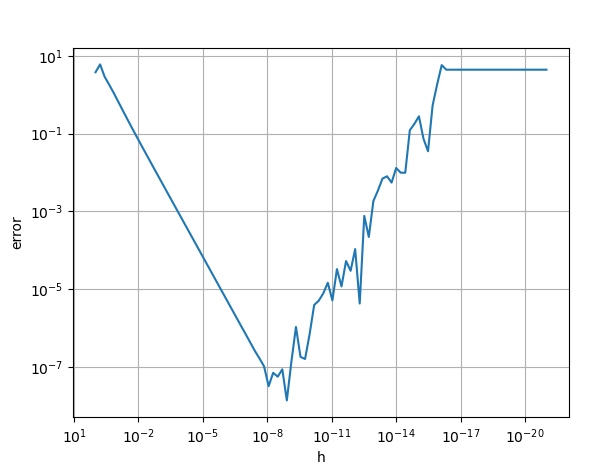
\includegraphics[width=0.5\textwidth]{fig/4ai.png}

                            \item \texttt{py output: min e of 2.7182700534922333e-11 at h = 1.1497569953977361e-06} \\
                                  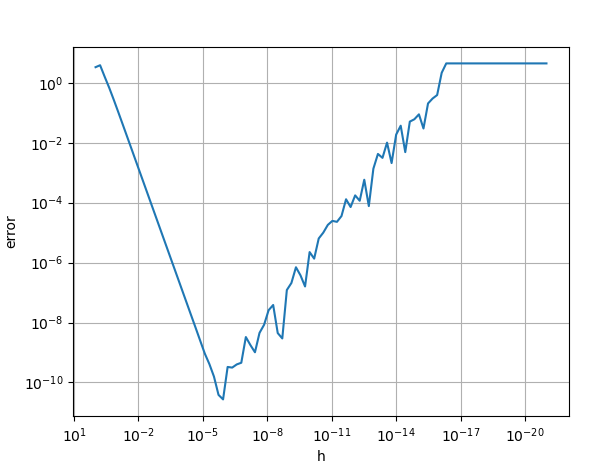
\includegraphics[width=0.5\textwidth]{fig/4aii.png}

                            \item \texttt{py output: min e of 4.330683012199188e-08 at h = 2.1544346900318827e-05} \\
                                  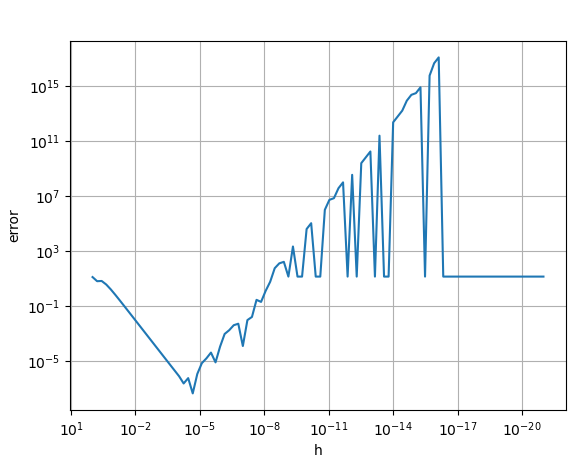
\includegraphics[width=0.5\textwidth]{fig/4aiii.png}
                        \end{enumerate}
                  \item
                        \begin{enumerate}
                            \item
                                  \texttt{py output: For a subinterval of 10, intergral is 4.607872940794085} \\
                                  \texttt{py output: For a subinterval of 20, intergral is 4.651934278080257}\\
                                  \texttt{py output: For a subinterval of 40, intergral is 4.664330479310646}\\
                                  \texttt{py output: For a subinterval of 80, intergral is 4.667686103287532}\\
                                  \texttt{py output: For a subinterval of 160, intergral is 4.668571606382887}\\
                                  Therefore the interval can be estimated to converge on \textbf{4.669} \\
                                  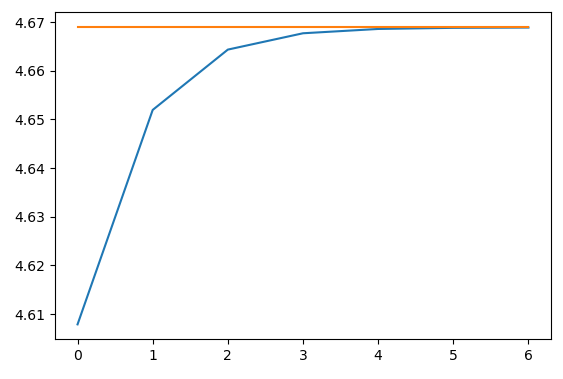
\includegraphics[width=0.5\textwidth]{fig/4bi.png}
                            \item
                                  \texttt{py output: For a subinterval of 10, intergral is 4.657102287466295}\\
                                  \texttt{py output: For a subinterval of 20, intergral is 4.666621390508981}\\
                                  \texttt{py output: For a subinterval of 40, intergral is 4.668462546387442}\\
                                  \texttt{py output: For a subinterval of 80, intergral is 4.668804644613161}\\
                                  \texttt{py output: For a subinterval of 160, intergral is 4.668866774081337}\\
                                  Giving the speed of conversion, a comfortable approximation is 4dp after 5 iterations: \textbf{6.6689}
                                  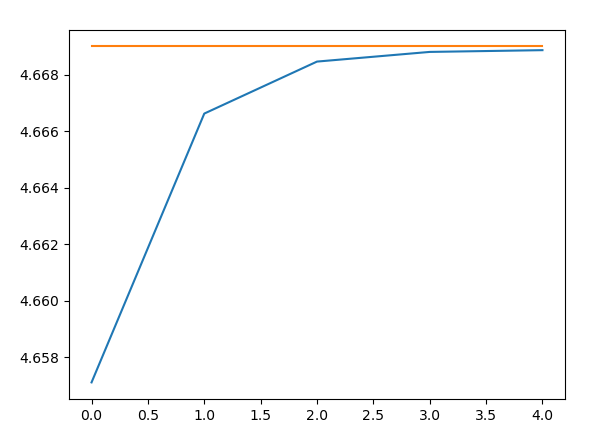
\includegraphics[width=0.5\textwidth]{fig/4bii.png}
                            \item
                                  \texttt{py output: output at upperlimit: 10 = 4.668880328350932}\\
                                  \texttt{py output: output at upperlimit: 100 = 11.875967391881685}\\
                                  \texttt{py output: output at upperlimit: 1000 = 11.999999998713985}\\
                                  This appears to be converging on 12\\
                                  \texttt{py output: To positive infinity: 12.000000000094914} \\
                                  With some floating point error, this confirms 12.
                        \end{enumerate}
              \end{enumerate}
    \end{enumerate}

\end{preview}
\begin{preview}
    
    \lstinputlisting[language=Python]{engr222_ass2_eisendani.py}

\end{preview}

\end{document}